\documentclass[titlepage, a4paper, openbib, 10pt]{article}

%#####################################
%Usepackages en installingen
\usepackage[top=1in, bottom=1in, left=1in, right=1in]{geometry}
\usepackage[pdftex]{graphicx}
\usepackage{fancyhdr}
\usepackage{sectionbox}
\usepackage[english]{babel}

\usepackage{chngcntr}
\usepackage{cite}
\usepackage{url}
\usepackage{makeidx}
\usepackage{paralist}
\usepackage{enumitem}
\usepackage{tocloft}
\usepackage{listliketab}	
\usepackage[table]{xcolor}
\usepackage{tabularx}
\usepackage{epsfig}
\usepackage{pdflscape}
\usepackage{pdfpages}
\usepackage{float}
\usepackage{multirow} 
\usepackage{rotating}
\usepackage[utf8]{inputenc}
\usepackage{color}
\usepackage{fp}
\usepackage[hidelinks]{hyperref}
\hypersetup{
    colorlinks=false,
    linkcolor=black,
    filecolor=black,
    urlcolor=black,
}
%\usepackage{draftwatermark}
%\SetWatermarkText{\textsc{Draft}}
%\SetWatermarkScale{5}
\newcommand{\red}[1]{
\textcolor{red}{#1}
}

\usepackage{tikz}

\usepackage{listings}
\lstset{language=C,
basicstyle=\ttfamily\footnotesize,
frame=shadowbox,
mathescape=true,
showstringspaces=false,
showspaces=false,
breaklines=true}

%#####################################
%Glossary
%\usepackage{glossaries}
\usepackage[toc,nonumberlist,nopostdot]{glossaries}
\makeglossaries


\newglossaryentry{assignment}{name=Assignment, description={
    A large-sized task to be completed by a student in order to get a grade.
    Assignments are related to learning objectives.
    Students are expected to show their skill and understanding of those learning objectives within an assignment.}}

\newglossaryentry{exercise}{name=Exercise, description={
    A small- to medium-sized task to be completed by a student in order to gain experience, understanding and feedback. }}

\newglossaryentry{exam}{name=Theoretical exam, description={The summative assessment at the end of the course. Scoring $>=5.5$ is a strict condition for being rewarded credit points. (Dutch: tentamen).}}

\newglossaryentry{oral}{name=Oral check, description={The summative assessment at the end of the course, determining the final grade.}}

\newglossaryentry{competence}{name=Competence, description={A brief description of what students are expected to learn during the study programme (informatica).}}

\newglossaryentry{lo}{name=Learning objective, description={
    A brief description of what students are expected to learn during the course.
    In general, each course has between 1 and 10 learning objectives.}}

%\newglossaryentry{to}{name=Task objective, description={A brief description of what students are expected to learn during a task.}}

\newglossaryentry{feedback}{name=Feedback, description={
    "... feedback is conceptualized as information provided by an agent
    (e.g., teacher, peer, book, parent, self, experience) regarding aspects of one’s per- formance or understanding.
    A teacher or parent can provide corrective information, a peer can provide an alternative strategy,
    a book can provide information to clarify ideas, a parent can provide encouragement,
    and a learner can look up the answer to evaluate the correctness of a response.
    Feedback thus is a “consequence” of performance." \footnote{Hattie, J., \& Timperley, H. (2007). The Power of Feedback. Review of Educational Research, 77(1), 81–-112.}}
    }

\newglossaryentry{undbeh}{
	name=UNDBEH
	, description={The \Gls{lo} stating that at the end of this course: the student has \textbf{understood} the behavioural design patterns.}
	, first= {has \textbf{understood} the behavioural design patterns. \texttt{UNDBEH}}
	, symbol=\texttt{UNDBEH}
}

\newglossaryentry{impbeh}{
	name=IMPBEH
	, description={The \Gls{lo} stating that at the end of this course: the student can \textbf{implement} the behavioural design patterns.}
	, first= {can \textbf{implement} the behavioural design patterns. \texttt{IMPBEH}}
	, symbol=\texttt{IMPBEH}
}

\newglossaryentry{undstr}{
	name=UNDSTR
	, description={The \Gls{lo} stating that at the end of this course: the student has \textbf{understood} the structural design patterns.}
	, first= {has \textbf{understood} the structural design patterns. \texttt{UNDSTR}}
	, symbol=\texttt{UNDSTR}
}

\newglossaryentry{impstr}{
	name=IMPSTR
	, description={The \Gls{lo} stating that at the end of this course: the student can \textbf{implement} the structural design patterns.}
	, first = {can \textbf{implement} the structural design patterns. \texttt{IMPSTR}}
	, symbol=\texttt{IMPSTR}
}

\newglossaryentry{undcre}{
	name=UNDCRE
	, description={The \Gls{lo} stating that at the end of this course: the student has \textbf{understood} the creational design patterns.}
	, first= {has \textbf{understood} the creational design patterns. \texttt{UNDCRE}}
	, symbol=\texttt{UNDCRE}
}

\newglossaryentry{impcre}{
	name=IMPCRE
	, description={The \Gls{lo} stating that at the end of this course: the student can \textbf{implement} the creational design patterns.}
	, first= {can \textbf{implement} the creational design patterns. \texttt{IMPCRE}}
	, symbol=\texttt{IMPCRE}
}


\newglossaryentry{abs}{
      name=ABS
    , description={The \Gls{lo} stating that at the end of this course: the student \textbf{is able to use} and \textbf{create} interfaces and abstract classes.}
    , first={\textbf{is able to use} and \textbf{create} interfaces and abstract classes. \texttt{(ABS)}}
    , symbol=\texttt{ABS}
    }
\newglossaryentry{learn}{
      name=LEARN
    , description={The \Gls{lo} stating that at the end of this course: the student \textbf{has developed skills} to adopt a new programming language with little support.}
    , first={\textbf{has developed skills} to adopt a new programming language with little support. \texttt{(LEARN)}}
    , symbol=\texttt{LEARN}
    }
\newglossaryentry{enc}{
      name=ENC
    , description={The \Gls{lo} stating that at the end of this course: the student \textbf{is able to apply} the concepts of data encapsulation, inheritance, and polymorphism to software.}
    , first={\textbf{is able to apply} the concepts of data encapsulation, inheritance, and polymorphism to software. \texttt{(ENC)}}
    , symbol=\texttt{ENC}
    }
\newglossaryentry{type}{
      name=TYPE
    , description={The \Gls{lo} stating that at the end of this course: the student \textbf{can apply} the concepts of data types.}
    , first={\textbf{can apply} the concepts of data types. \texttt{(TYPE)}}
    , symbol=\texttt{TYPE}
    }
\newglossaryentry{bhf}{
      name=BHF
    , description={The \Gls{lo} stating that at the end of this course: the student \textbf{understands} basic human factors.}
    , first={\textbf{understands} basic human factors. \texttt{(BHF)}}
    , symbol=\texttt{BHF}
    }

%\loadglsentries{Glossary}


%\usepackage{showframe} %tmp
%#####################################
%Nieuwe commando's
\newcommand{\HRule}{\rule{\linewidth}{1pt}}
\newcommand{\organisatie}{\uppercase{Hogeschool Rotterdam / CMI}}
\newcommand{\modulenaam}{Development 4}
\newcommand{\modulecode}{\uppercase{INFDEV02-4}}
\newcommand{\studiejaar}{\uppercase{2016-2017}}
\newcommand{\stdPunten}{4}
\renewcommand{\author}{The DEV team}

\definecolor{lichtGrijs}{RGB}{169,169,169}



%#####################################
%Index en styling
\setlength{\cftbeforesecskip}{10pt}
\setlength\parindent{0pt}
\makeindex
\graphicspath{{../Img/}}
\counterwithin{figure}{subsection}
\pagestyle{fancy}
\setcounter{secnumdepth}{5}
\setcounter{tocdepth}{5}

%#####################################
%     Alles voor header/footer
\fancyhf[HL]{\nouppercase{\textit{\leftmark}}}
\setlength{\headheight}{36pt}
\lhead{\uppercase{\footnotesize Course description}}
\chead{\footnotesize \organisatie}
\rhead{
\includegraphics[width=0.09\textwidth]{logo}}

\lfoot{\scriptsize \modulenaam}
\cfoot{\scriptsize \today}
\rfoot{\small \thepage}

\renewcommand{\headrulewidth}{0.4pt}
\renewcommand{\footrulewidth}{0.4pt}
%#####################################

\begin{document}


%#####################################
%Titlepage
\begin{titlepage}
\thispagestyle{fancy}
\ 
\vspace{5cm}

\begin{center}

	
	\Large \textbf \organisatie
	
	\vspace{1.5cm}
	
	\HRule \\[0.4cm]
	
	\Huge \textbf \modulenaam
	
	\vspace{1.7cm}
	
	\Large \textbf  \modulecode \\
	\studiejaar
	
	\vspace{0.4cm}
	
	\HRule \\[1.5cm]
\end{center}
\vfill

% Author and supervisor
\begin{tabular}{l l}
	Number of study points:  & \stdPunten{} ects\\
	Course owners: & \author\\
\end{tabular}


\end{titlepage}

%####### Contentpagina ########
%\renewcommand{\baselinestretch}{1.5}\normalsize
%\tableofcontents
%\newpage
%\listoffigures
%\newpage
%\listoftables
%\newpage

%########### Inhoud ###########

\shadowsectionbox
\section*{Module description}
\begin{tabularx}{\textwidth}{|>{\columncolor{lichtGrijs}} p{.26\textwidth}|X|}
	\hline
	\textbf{Module name:} & \modulenaam\\

	\hline
	\textbf{Module code: }& \modulecode\\
	\hline
	\textbf{Study points \newline and hours of effort:} & This module gives \stdPunten{}  ects, in correspondence with \FPeval{\result}{clip(\stdPunten*28)}\result{} hours:
	\begin{itemize}
		\item 2 X 3 x 6 hours of combined lecture and practical
		\item the rest is self-study
	\end{itemize} \\
	\hline
	\textbf{Examination:} & Written examination and practicums (with oral check) \\
	\hline
	\textbf{Course structure:} & Lectures, self-study, and practicums \\
	\hline
	\textbf{Prerequisite knowledge:} & INFDEV02-1, INFDEV02-2, and INFDEV02-3. \\
	\hline
	\textbf{Learning materials:}  &
		\begin{itemize}
			\item Book: Design patterns, elements of reusable object-oriented software; author Erich Gamma, Richard Helm, Ralph Johnson, John Vlissides.
			\item Slides: found on N@tschool and on the GitHub repository \href{https://github.com/hogeschool/INFDEV02-4}{github.com/hogeschool/INFDEV02-4}
			\item \Glspl{exercise} and \glspl{assignment}, to be done at home and during practical part of the lectures (pdf): found on N@tschool and on the GitHub repository \href{https://github.com/hogeschool/INFDEV02-4}{github.com/hogeschool/INFDEV02-4}
		\end{itemize} \\
	\hline
	\textbf{Connected to competences:} & realiseren en ontwerpen \\
	\hline
	\textbf{Learning objectives:} &
		At the end of the course, the student:
			\begin{itemize}
                \item \glsfirst{undbeh}
                \item \glsfirst{impbeh}
                \item \glsfirst{undstr}
                \item \glsfirst{impstr}
                \item \glsfirst{undcre}
                \item \glsfirst{impcre}
			\end{itemize} \\
	\hline
%\end{tabularx}
%\newpage
%
%\begin{tabularx}{\textwidth}{|>{\columncolor{lichtGrijs}} p{.26\textwidth}|X|}
%	\hline
%	\textbf{Content:}&
%	\begin{itemize}
%		\item _
%	\end{itemize} \\
%	\hline
	\textbf{Course owners:} & \author\\
	\hline
	\textbf{Date:} & \today \\
	\hline
\end{tabularx}
%\newpage


\newpage
\section{General description}
		Designing a object-oriented software is a complex and time-consuming task. A misuse of typical object-oriented language features, such as polymorphism or inheritance, cause errors and inflexible solutions. Design patterns provide the means to write code which is both maintainable and re-usable. \\
		

	\subsection{Relationship with other teaching units}
		Subsequent programming courses build upon the knowledge learned during this course.	\\		
		Knowledge acquired through the programming courses is also useful for the projects. A word of warning though: projects and development courses are largely independent, so some things that a student learns during the development courses are not used in the projects, some things that a student learns during the development courses are indeed used in the projects, but some things done in the projects are learned within the context of the project and not within the development courses.


%\newpage
\section{Course program}
The course is structured into six lectures.
The six lectures take place during the course, but are not necessarily in a one-to-one correspondence with the course weeks.

\subsection{Chapter 0 - reuse through generics}
\paragraph*{Topics}			
\begin{itemize}
	\item Using generic parameters
	\item (\textbf{Advanced}) Using covariance and contravariance in the presence of generic parameters
	\item (\textbf{Advanced}) Designing interfaces and implementation in the presence of generic parameters
\end{itemize}

\subsection{Chapter 1 - Intro to design patterns} 
\paragraph*{Topics}
\begin{itemize}
	\item What are design patterns? \glssymbol{undbeh}
	\item Visiting polymorphic instances. \glssymbol{impbeh}
	\item Pure object-oriented Visitor pattern \glssymbol{impbeh}
	\item Functional approach to Visitor pattern \glssymbol{impbeh}
\end{itemize}

\subsection{Chapter 2 - Iterating collections}
\paragraph*{Topics}			
\begin{itemize}
	\item What is an iterator? \glssymbol{undbeh}
	\item Why using iterators? \glssymbol{undbeh}
	\item Iterating a generic collection. \glssymbol{impbeh}
\end{itemize}

\subsection{Chapter 3 - Extending behaviours}
\paragraph*{Topics}			
\begin{itemize}
	\item Decorator pattern. \glssymbol{undstr}
	\item Decorating over iterator. \glssymbol{impstr}
\end{itemize}


\subsection{Chapter 4 - Entity construction}
\paragraph*{Topics}			
\begin{itemize}
	\item Creating object without specifying the class type. \glssymbol{undcre}, \glssymbol{impcre}
\end{itemize}


\subsection{Chapter 5 - Adapting behaviours}
\paragraph*{Topics}			
\begin{itemize}
	\item Managing different objects with shared behaviours. \glssymbol{undstr}
	\item Adapter pattern. \glssymbol{impstr}
\end{itemize}
\newpage
\section{Assessment}
The course is tested with two exams:
A series of \glspl{assignment} which have to be handed in, but won't be graded. There will be an \gls{oral}, which is based on the \glspl{assignment}
and a written exam. The final grade is determined as follows: \\

\texttt{if \gls{exam}-grade $ >= 5.5 $ then return \gls{oral}-grade else return 0}

\paragraph*{Motivation for grade}
A professional software developer is required to be able to program code which is, at the very least, \textit{correct}.

In order to produce correct code, we expect students to show:
\begin{inparaenum}[\itshape i\upshape)]
\item a foundation of knowledge about how a programming language actually works in connection with a simplified concrete model of a computer;
\item fluency when actually writing the code.
\end{inparaenum}

The quality of the programmer is ultimately determined by his actual code-writing skills, therefore the written exam will require you to write code; this ensures that each student is able to show that his work is his own and that he has adequate understanding of its mechanisms.


\subsection{Theoretical examination \modulecode}
The general shape of a \gls{exam} for \texttt{\modulecode} is made up of a short series of highly structured open questions.
In each exam the content of the questions will change, but the structure of the questions will remain the same.
For the structure (and an example) of the theoretical exam, see the appendix.


\subsection{Practical examination \modulecode}
There is one \glspl{assignment} that is mandatory.

The assignment asks you to implement a GUI system in the fashion of Windows Form with an immediate drawing library, such as Monogame. In the assignment you have to show that you can use effectively some of the design patterns learnt during the course. Your GUI library should allow to create at least clickable buttons and text labels organized in a single panel. Optionally you can implement a system with a scrollable panel. You are free to choose the implementation details as long as you show the usage of design patterns. Each design pattern that it is correctly use will increase the grade of the assignment (see below for further details).

\begin{itemize}
  \item All assignments are to be presented at the end of the oral assessment to the teacher upon request
  \item Each assignment is designed to assess the students knowledge related to one or more \glspl{lo}.
          If the teacher is unable to assess the students' ability related to the appropriate \gls{lo} based on his work, then no points will be awarded for that part.
  \item At the oral check you will be given 1 point for each design pattern learnt in class which is used \textit{appropriately} in your assignment to a maximum of 4 points. At the oral check you will be asked to solve one ore more exercises on design patterns. The maximum score for this part is up to 6 points. The final grade for the oral check will be the sum of the points for the assignment and the one for the exercises.
  \begin{itemize}
  	\item The design patterns used for the assignment should be those seen in the course: visitor, decorator, abstract, iterator, and adapter.
  	\item Factories can be used to abstract away the creation of elements of the form.
  	\item Decorators can be used to extend the behaviors of GUI controls
  	\item Etc..  	
  \end{itemize}
  \item \textit{The teachers still reserve the right to check the practicums handed in by each student, and to use it for further evaluation.}
  \item The university rules on fraude and plagiarism (Hogeschoolgids art. 11.10 -- 11.12) also apply to code;
\end{itemize}

\newpage
\section*{Structure of exam \modulecode}
The general shape of a theoretical exam for \texttt{\modulecode} is made up of highly structured open questions.

\paragraph{Question 1: } \ \\

\textbf{General shape of the question:} \textit{Given the following class definitions, and a piece of code that uses them, fill in the stack, heap, and PC with all steps taken by the program at runtime.}

\textbf{Concrete example of question:}

\lstset{numbers=left,basicstyle=\ttfamily\small}\lstset{language=[Sharp]C}
\begin{lstlisting}
public interface Option<T>
{

  U Visit<U>(Func<U> onNone, Func<T, U> onSome);
}
public class Some<T> : Option<T>
{
  T value;
  public Some(T value) { this.value = value; }
  public U Visit<U>(Func<U> onNone, Func<T, U> onSome)
  {
    return onSome(value);
  }
}
public class None<T> : Option<T>
{
  public U Visit<U>(Func<U> onNone, Func<T, U> onSome)
  {
    return onNone();
  }
}
...
Option<int> number = new Some<int>(5);
int inc_number = number.Visit(() => { throw new Exception("Expecting a value..."); }, i => i + 1);
Console.WriteLine(inc_number);
\end{lstlisting}
\textbf{Points:} \textit{3 (30\% of total).}

\textbf{Grading:} \textit{one point per correctly filled-in execution step.}

\textbf{Associated learning objective:} \glsfirst{impbeh}

\ \\ 

\paragraph{Question 2: } \ \\

\textbf{General shape of question:} \textit{Given the following class definitions, and a piece of code that uses them, fill in the declarations, class definitions, and PC with all steps taken by the compiler while type checking.}

\textbf{Concrete example of question:} 

\lstset{numbers=left,basicstyle=\ttfamily\small}\lstset{language=[Sharp]C}
\begin{lstlisting}
public interface Option<T>
{
  U Visit<U>(Func<U> onNone, Func<T, U> onSome);
}
public class Some<T> : Option<T>
{
  T value;
  public Some(T value) { this.value = value; }
  public U Visit<U>(Func<U> onNone, Func<T, U> onSome)
  {
    return onSome(value);
  }
}
public class None<T> : Option<T>
{
  public U Visit<U>(Func<U> onNone, Func<T, U> onSome)
  {
    return onNone();
  }
}
...
Option<int> number = new Some<int>(5);
int inc_number = number.Visit(() => { throw new Exception("Expecting a value..."); }, i => i + 1);
Console.WriteLine(inc_number);
\end{lstlisting}

\textbf{Points:} \textit{3 (30\% of total).}

\textbf{Grading:} \textit{Grading: one point per correctly filled-in type checking step.}

\textbf{Associated learning objective:} \glsfirst{undbeh}

\paragraph{Question 3: }

\textbf{General shape of question:} \textit{Given the following UML diagram of a design pattern, fill in the missing parts.}

\textbf{Concrete example of question:} 

\begin{center}
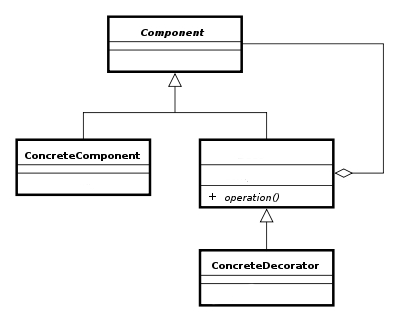
\includegraphics[width=\textwidth / 2]{decorator_uml}
\end{center}

\textbf{Points:} \textit{4 (40\% of total).}

\textbf{Grading:} \textit{Grading: one point per correctly filled-in block of code.}

\textbf{Associated learning objective:} \glsfirst{abs}

\ \\

\newpage

\newpage
%\bibliographystyle{plain}
%\bibliography{references}
\glossarystyle{altlist}
\printglossaries
\newpage

\section*{Appendix 1: Assessment matrix}
	\begin{tabular}{|p{2cm}|p{4cm}|}
		\hline
		\glssymbol{lo} & Dublin descriptors \\
		\hline
        \glssymbol{undbeh} & 1, 4, 5\\
        \hline
        \glssymbol{impbeh}& 2, 3, 5\\
        \hline
        \glssymbol{undstr} & 1, 4, 5\\
        \hline
        \glssymbol{impstr}& 2, 3, 5\\
        \hline
        \glssymbol{undcre} & 1, 4, 5\\
        \hline
        \glssymbol{impcre}& 2, 3, 5\\
        \hline
	\end{tabular}
	
	\vspace{1cm}

	Dublin-descriptors:
	\begin{enumerate}
		\item Knowledge and understanding
		\item Applying knowledge and understanding
		\item Making judgments
		\item Communication
		\item Learning skills
	\end{enumerate}


%\newpage
%\input{tex/Bijlage2}
%\newpage
%\input{tex/Bijlage3}
\printindex


\end{document}

